\documentclass{article}

\pdfminorversion=4

\usepackage{tikz}
\usetikzlibrary{fit,patterns,decorations.pathreplacing}

\usepackage[T1,T2A]{fontenc}
\usepackage[utf8]{inputenc}
\usepackage[russian,english]{babel} %Last language is default and active.
\usepackage{graphicx}

\def\thindivider{\centerline{\tiny%%
-- --- --- -- ~~~ --- --- --- ~~~ --- -- --- -- ~~~~~~
--- --- --- ~~~  -- --- -- ~~~~~~
--- --- -- ~~~ --- ~~~ -- -- --- -- ~~~ --- --- ---}}

\begin{document}

\title{This PDF is a Git Repository\\Containing its Own \LaTeX\ Source}
\author{Evan Sultanik}
\date{April 11, 2017}

\maketitle

Have you ever heard of the \texttt{git bundle} command? I hadn't. It
bundles a set of Git objects---potentially even an entire
repository---into a single file. Git allows you to treat that file as
if it were a standard Git database, so you can do things like clone a
repo directly from it. Its purpose is to easily sneakernet pushes or
even whole repositories across air gaps.

\thindivider

Neighbors, it's possible to create a PDF that is also a Git
repository.

\begin{center}
\begingroup
\setbox9=\hbox{\footnotesize\verb|Receiving objects: 100% (174/174), 103.48 KiB | 0 bytes/s, done.|}
\begin{minipage}{\wd9}
\footnotesize\begin{verbatim}
$ git clone article.pdf foo
Cloning into 'foo'...
Receiving objects: 100% (174/174), 103.48 KiB | 0 bytes/s, done.
Resolving deltas: 100% (100/100), done.
$ cd foo
$ ls
article.tex
article.pdf
\end{verbatim}
\end{minipage}
\endgroup
\end{center}

\section{The Git Bundle File Format}

The file format for Git bundles doesn't appear to be formally
specified anywhere, however, inspecting \texttt{bundle.c} reveals that
it's relatively straightforward:
\def\returnkey{\hspace*{1pt}{\setbox9=\hbox{$\hookleftarrow$}\tikz\node[text width=\wd9,fill=lightgray,rounded corners=1pt] at (0,0){$\hookleftarrow$};}\hspace*{1pt}}
\begin{center}
\begin{tikzpicture}
  \node[text width=0.9\hsize] at (0,0) (sig) {\footnotesize\tt\# v2 git bundle{\tiny\returnkey}};
  \node[inner sep=0mm,fit=(sig),draw,rounded corners,dashed,minimum width=0.9\hsize] (sigbox) {};
  \node[draw,rounded corners,fill=white] at (sigbox.north) (siglabel) {\footnotesize Git Bundle Signature};
  \node[text width=0.9\hsize,anchor=north west,yshift=-0.5mm] at (sig.south west) (b1) {\footnotesize\tt 3aa340a2e3d125ab6703e5c9bdfede2054a9c0c5 refs/heads/master{\tiny\returnkey}};
  \node[text width=0.9\hsize,anchor=north west,yshift=-0.5mm] at (b1.south west) (b2) {\footnotesize\tt 3aa340a2e3d125ab6703e5c9bdfede2054a9c0c5 refs/remotes/origin/master{\tiny\returnkey}};
  \node[text width=0.9\hsize,anchor=north west,yshift=-0.5mm] at (b2.south west) (b3) {\footnotesize\tt 4146cfe2fe9249fc14623f832587efe197ef5d2d refs/stash{\tiny\returnkey}};
  \node[text width=0.9\hsize,anchor=north west,yshift=-0.5mm] at (b3.south west) (b4) {\footnotesize\tt babdda4735ef164b7023be3545860d8b0bae250a HEAD{\tiny\returnkey}};
  \node[inner sep=0mm,fit=(b1) (b4),draw,rounded corners,dashed,minimum width=0.9\hsize] (digestbox) {};
  \node[rotate=-90,draw,rounded corners,fill=white] at (digestbox.east) {\footnotesize Digest};
  \node[text width=0.9\hsize,anchor=north west,yshift=-0.5mm] at (b4.south west) (empty) {{\tiny\returnkey}\footnotesize\ };
  \node[text width=0.9\hsize,anchor=north west,yshift=-0.5mm] at (empty.south west) (pack) {{\footnotesize\tt PACK}$\ldots$};
  \node[inner sep=0mm,fit=(pack),draw,rounded corners,dashed,minimum width=0.9\hsize] (packbox) {};
  \node[draw,rounded corners,fill=white] at (pack.south) {\footnotesize Git Packfile};
\end{tikzpicture}
\end{center}
Git uses its Packfile format to compress the objects in its database,
as well as to reduce network bandwidth when pushing and pulling, which
makes it an obvious choice for use inside bundles. This of course
raises the question: What is the format for a Git Packfile?

Git does have some internal documentation in
\begin{center}
  \texttt{Documentation/technical/pack-format.txt}
\end{center}
however, it is rather sparse, and does not provide enough detail to
fully parse the format. The documentation also has some
``observations'' that suggest it wasn't even written by the file
format's creator and instead was written by a developer who was later
trying to make sense of the code.

Luckily, Aditya Mukerjee already had to reverse engineer the file
format for his GitGo clean-room implementation of Git, and he wrote an
excellent blog entry about
it\footnote{\texttt{https://codewords.recurse.com/issues/three/unpacking-git-packfiles}}.

\begin{center}
{\small
\def\char#1{\,`\texttt{#1}'\,}
\setbox9=\hbox{\char{K}}
\newdimen\bytewidth\bytewidth=\wd9
\def\byte#1{\hbox to \bytewidth{\hfil\texttt{#1}\hfil}}
\def\desc#1#2{\hbox to #1\bytewidth{\hfil #2\hfil}}
\def\underbrace#1{\draw [
    thick,
    decoration={
        brace,
        mirror,
        raise=2pt
    },
    decorate
] ([xshift=1pt]#1.base west) -- ([xshift=-1pt]#1.base east) 
node (#1label) [pos=0.5,anchor=north,yshift=-2pt]}
\begin{tikzpicture}
\node[inner sep=0pt,minimum width=4\bytewidth] at (0,0) (pack) {\char{P}\char{A}\char{C}\char{K}};
\node[inner sep=0pt,anchor=base west] at (pack.base east) (version) {\byte{00}\byte{00}\byte{00}\byte{02}};
\node[inner sep=0pt,anchor=base west] at (version.base east) (numobj) {\desc{4}{\# objects}};
\underbrace{pack}{\tiny magic};
\underbrace{version}{\tiny version};
\underbrace{numobj}{\tiny big-endian 4 byte int};
\node[inner sep=0pt,anchor=north west] at (packlabel.south -| pack.west) (chunks) {one data chunk for each object};
\node[inner sep=0pt,anchor=north west] at ([yshift=-0.5\baselineskip]chunks.south west) (sha1) {20-byte SHA-1 of all the previous data in the pack};
\end{tikzpicture}}
\end{center}

I hope you like Soviet holes, dear neighbor, because chasing this
rabbit might remind you of \foreignlanguage{russian}{Кольская}. If you
grew bored reading Tristram Shandy, it's safe to skip to the next
section, 'cause it's turtles all the way down.

\begin{center}
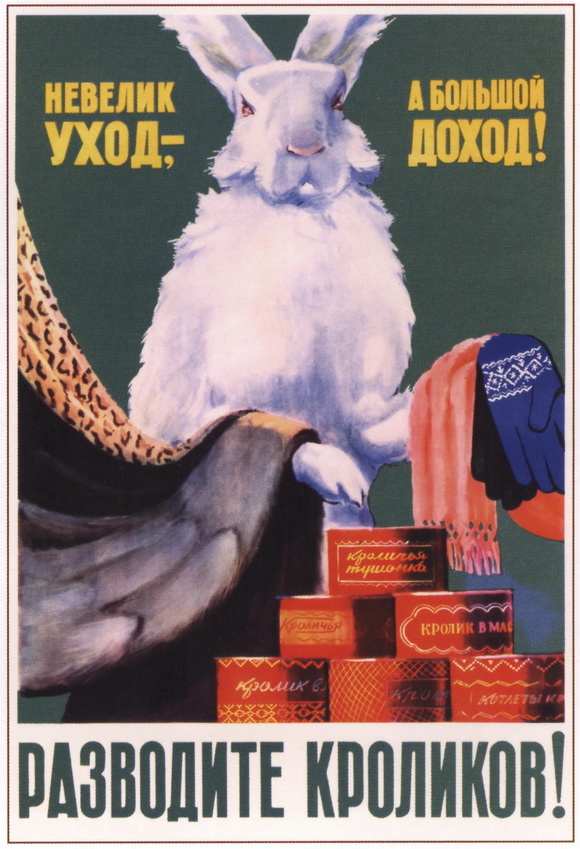
\includegraphics[width=0.5\hsize]{RazvodityeKrolikov}
\end{center}

Okay, the next step is to figure out the ``chunk'' format.  The chunk
header is variable length, and can be as small as one byte. It encodes
the type of object and the \emph{uncompressed} size of the object. If
the object is a \textit{delta} (\textit{i.e.}, a diff, as opposed to a
complete object), the header is followed by either the SHA-1 hash of
the base object to which the delta should be applied, or a byte
reference within the packfile for the start of the base object. The
remainder of the chunk consists of the object data, zlib-compressed.
\begin{center}
{\newcount\bitnum\bitnum=0
\begin{tikzpicture}
\node[coordinate] at (0,0) (b0) {};
\foreach \i in {1,0,1,1,0,1,0,0,0,1,0,1,0,1,1,0} {
  {\newcount\prevbit\prevbit=\bitnum
  \global\advance\bitnum by 1
  \node[anchor=west] at (b\the\prevbit.east) (b\the\bitnum) {\i};}
  \draw ([xshift=1pt]b\the\bitnum.south west) -- ([xshift=-1pt]b\the\bitnum.south east);
}
\end{tikzpicture}}
\end{center}

\end{document}
